%% abtex2-modelo-trabalho-academico.tex, v-1.9.6 laurocesar
%% Copyright 2012-2016 by abnTeX2 group at http://www.abntex.net.br/ 
%%
%% This work may be distributed and/or modified under the
%% conditions of the LaTeX Project Public License, either version 1.3
%% of this license or (at your option) any later version.
%% The latest version of this license is in
%%   http://www.latex-project.org/lppl.txt
%% and version 1.3 or later is part of all distributions of LaTeX
%% version 2005/12/01 or later.
%%
%% This work has the LPPL maintenance status `maintained'.
%% 
%% The Current Maintainer of this work is the abnTeX2 team, led
%% by Lauro César Araujo. Further information are available on 
%% http://www.abntex.net.br/
%%
%% This work consists of the files abntex2-modelo-trabalho-academico.tex,
%% abntex2-modelo-include-comandos and abntex2-modelo-references.bib
%%

% ------------------------------------------------------------------------
% ------------------------------------------------------------------------
% abnTeX2: Modelo de Trabalho Academico (tese de doutorado, dissertacao de
% mestrado e trabalhos monograficos em geral) em conformidade com 
% ABNT NBR 14724:2011: Informacao e documentacao - Trabalhos academicos -
% Apresentacao
% ------------------------------------------------------------------------
% ------------------------------------------------------------------------

\documentclass[
	% -- opções da classe memoir --
	12pt,				% tamanho da fonte
	openright,			% capítulos começam em pág ímpar (insere página vazia caso preciso)
	oneside,			% para impressão em recto e verso. Oposto a oneside
	a4paper,			% tamanho do papel. 
	% -- opções da classe abntex2 --
	%chapter=TITLE,		% títulos de capítulos convertidos em letras maiúsculas
	%section=TITLE,		% títulos de seções convertidos em letras maiúsculas
	%subsection=TITLE,	% títulos de subseções convertidos em letras maiúsculas
	%subsubsection=TITLE,% títulos de subsubseções convertidos em letras maiúsculas
	% -- opções do pacote babel --
	english,			% idioma adicional para hifenização
	spanish,			% idioma adicional para hifenização
	brazil				% o último idioma é o principal do documento
	]{abntex2}

% ---
% Pacotes básicos 
% ---
\usepackage{lmodern}			% Usa a fonte Latin Modern	
\usepackage[T1]{fontenc}       % Selecao de codigos de fonte.		
\usepackage[utf8]{inputenc}		% Codificacao do documento (conversão automática dos acentos)
\usepackage{lastpage}			% Usado pela Ficha catalográfica
\usepackage{indentfirst}		% Indenta o primeiro parágrafo de cada seção.
\usepackage{color}				% Controle das cores
\usepackage{graphicx}			% Inclusão de gráficos
\usepackage{microtype} 			% para melhorias de justificação
\usepackage{mathtools}

% ---

% ---
% Pacotes de citações
% ---
\usepackage[brazilian,hyperpageref]{backref}	 % Paginas com as citações na bibl
\usepackage[alf]{abntex2cite}	% Citações padrão ABNT

% --- 
% CONFIGURAÇÕES DE PACOTES
% --- 

% ---
% Configurações do pacote backref
% Usado sem a opção hyperpageref de backref
\renewcommand{\backrefpagesname}{Citado na(s) página(s):~}
% Texto padrão antes do número das páginas
\renewcommand{\backref}{}
% Define os textos da citação
\renewcommand*{\backrefalt}[4]{
	\ifcase #1 %
		Nenhuma citação no texto.%
	\or
		Citado na página #2.%
	\else
		Citado #1 vezes nas páginas #2.%
	\fi}%
	
	
\graphicspath{ {images/} }

% ---


% ---
% Informações de dados para CAPA e FOLHA DE ROSTO
% ---
\titulo{Protótipo de um sistema para análise de sentimentos em redes sociais usando computação cognitiva}
\data{2017}
\autor{Flavia Pezoti \and Aline Murakami \and Eric Campanatti \and Gabriel Alves }
\instituicao{Pontifícia Universidade Católica de São Paulo}
\local{São Paulo}
\orientador{}
\coorientador{}
\tipotrabalho{}
% O preambulo deve conter o tipo do trabalho, o objetivo, 
% o nome da instituição e a área de concentração 
\preambulo{}
% ---



% ---
% Configurações de aparência do PDF final

% informações do PDF
\makeatletter
\hypersetup{
     	%pagebackref=true,
		pdftitle={\@title}, 
		pdfauthor={\@author},
    	pdfsubject={\imprimirpreambulo},
	    pdfcreator={LaTeX with abnTeX2},
		pdfkeywords={abnt}{latex}{abntex}{abntex2}{trabalho acadêmico}, 
		colorlinks=true,       		% false: boxed links; true: colored links
    	linkcolor=black,          	% color of internal links
    	citecolor=black,        		% color of links to bibliography
    	filecolor=black,      		% color of file links
		urlcolor=black,
		bookmarksdepth=4
}
\makeatother
% --- 

% --- 
% Espaçamentos entre linhas e parágrafos 
% --- 

% O tamanho do parágrafo é dado por:
\setlength{\parindent}{1.3cm}

% Controle do espaçamento entre um parágrafo e outro:
\setlength{\parskip}{0.2cm}  % tente também \onelineskip

% ---
% compila o indice
% ---
\makeindex
% --
% ----
% Início do documento
% ----
\begin{document}

% ----------------------------------------------------------
% ELEMENTOS PRÉ-TEXTUAIS
% ----------------------------------------------------------

 \pretextual

% ---
% Capa
% ---
\imprimircapa
% ---

% ---
% inserir o sumario
% ---
\pdfbookmark[0]{\contentsname}{toc}
\tableofcontents*
\cleardoublepage
% ---


% ----------------------------------------------------------
% ELEMENTOS TEXTUAIS
% ----------------------------------------------------------
\textual

\chapter{Introdução}
	Neste capítulo serão apresentados os pontos que foram decisivos na escolha do tema do projeto, e também quais serão as atividades a serem efetuadas para alcançar os objetivos estabelecidos

	\section{Motivação}
	
	Atualmente, o uso de redes sociais, como Facebook, Twitter, Instagram e outros, ocupa uma parcela significante da rotina das pessoas. Bilhões de internautas as utilizam diariamente não apenas para entrar em contato com seus amigos, conhecer novas amizades e divulgar informações que julgam interessantes, mas também expressar e compartilhar, por meio de postagens, vídeos e fotos, seus pontos de vista a respeito de uma extensa gama de assuntos.
	
	Uma postagem criada por um usuário pode gerar muitas informações a respeito de seu estilo de vida: em qual cidade ele mora, onde costuma fazer compras, quais suas preferências musicais, etc. Estas informações extraídas da maneira correta se transformam em dados sociais. A crescente disponibilidade destes dados sociais é extremamente benéfica para tarefas como branding, análise de produtos, gerenciamento de reputação corporativa e marketing de mídia social \cite{article_sentiment_analysis}. 
	
No entanto, o volume de dados criado pelas redes sociais torna ineficiente que pessoas obtenham, pesquisem e classifiquem dados sem ajuda computacional \cite{conference_fb}. Além disso, a descoberta de informações úteis a partir desta enorme quantidade de dados não estruturados continua a ser um desafio aberto \cite{article_tweet_crisis}.

	A natureza complexa dos conteúdos compartilhados em redes sociais requer técnicas avançadas de aprendizado de máquina e processamento de linguagem natural, para que se possa extrair opiniões dos usuários sobre um determinado tema \cite{article_sentiment_twitter}.
Embora esses dados sejam facilmente compreensíveis aos seres humanos, eles não são adequados para o processamento automático: as máquinas ainda não conseguem interpretar de forma eficaz e dinâmica o significado associado ao texto em linguagem natural em ambientes muito grandes, heterogêneos, barulhentos e ambíguos como a Web \cite{article_sentiment_analysis}.

	Emular e compreender o cérebro humano é um dos principais desafios da inteligência computacional, que envolve muitos problemas-chave da inteligência artificial, incluindo a compreensão da linguagem humana, raciocínio e emoções. 
Dessa forma, com este trabalho procura-se compreender e aplicar técnicas de inteligência computacional e processamento linguístico para desenvolver um algoritmo capaz de entender e identificar sentimentos associados a textos de mídias sociais dentro de uma determinada temática. 
	
	\section{Objetivo}
	O objetivo deste trabalho é desenvolver o protótipo de um sistema capaz de identificar os sentimentos humanos expressados em postagens de redes sociais sobre um determinado tema.
	
	 Serão pré-determinados “grupos de sentimentos”, nos quais as postagens serão enquadradas a partir de indicadores linguísticos a serem estudados ao longo da pesquisa. A expectativa é que o sistema seja capaz de enquadrar os textos em sentimentos obtendo um resultado similar ao que uma pessoa teria realizando o processo manualmente.
	
Ao final do projeto, será realizada uma comparação dos resultados obtidos pelo algoritmo desenvolvido durante o trabalho com um algoritmo aleatório e com os resultados obtidos por ferramentas de computação cognitiva populares no cenário atual.	
	
	\section{Método de Trabalho}
	   
	   A pesquisa se dividirá em duas partes fundamentais: o estudo dos conceitos base que fundamentam o trabalho e o desenvolvimento de um algoritmo e de um protótipo, que colocam em prática os conhecimentos adquiridos durante este estudo. As macroatividades que compõem estão descritas abaixo.
		
		
		\subsection*{Pesquisa Bibliográfica}
		
				\begin{itemize}
					\item Levantamento de bibliografias que abordem os temas: Computação cognitiva, Machine learning, Natural Language Processing (NLP), Algoritmos de análise de emoções (Extreme Machine Learning - EML e Suport Vector Machine - SVM) e análises de postagens em redes sociais.
					\item Levantamento de trabalhos relacionados à temática desta pesqusa, a fim de localizar pontos que possam ser explorados ou estendidos durante a elaboração do projeto.
					
				\end{itemize}
				
		\subsection*{Estudo e Exploração Tecnológica dos Princípios de Inteligência Artifical }
				
				\begin{itemize} 
					\item Avaliação dos bancos de dados léxicos de análise de sentimentos (SentiWordNet, ConceptNet, SentiSense)
					\item Possibilidade de usar Watson (IBM) e/ou LEX (AWS) para análise dos dados
					\item Confecção do capítulo 2 do TCC, a partir dos tópicos pesquisados.
				\end{itemize}			
				
		\subsection*{Coleta dos Dados Iniciais}
		Realizar a análise de sentimentos de tweets requer uma base de dados. Para isso será feito um data mining de posts do Twitter que serão o conjunto inicial para a análise.
		 
				\begin{itemize}
					\item Datamining das postagens das redes sociais e armazenamento em um banco de dados para posterior análise. (WEKA \cite{article_weka} ou tweetstream \cite{tweetstream})
				\end{itemize}
				
		\subsection*{Desenvolvimento do Algoritmo para Análise de Sentimentos}				

				\begin{itemize}
					\item Análise dos algoritmos na literatura, adaptação e desenvolvimento de um algoritmo próprio para o escopo do problema.	Consistirá na análise de eficiência dos diferentes algoritmos para textos curtos e não estruturados. E, posteriormente, adaptação para alimentar uma base de dados do Watson.

					\item Treinamento do Algoritmo: Nesta fase o sistema é treinado com o uso de um conjunto de treinamento constituído por textos previamente classificados para obter a probabilidade de que uma palavra seja positiva, negativa ou neutra dada a classe atribuída ao texto.
					\item Teste do Algoritmo: O algoritmo é testado para calcular a precisão do método.
					\item Uso do Algoritmo: Nesta fase, a entrada do algoritmo é um conjunto de textos não classificados e é determinado se são positivos, negativos ou neutros.
				\end{itemize}
				
		\subsection*{Desenvolvimento do Protótipo}
		
		Nesta atividade, o protótipo de um sistema será modelado e implementado tendo como núcleo o algoritmo de análise de sentimentos desenvolvido anteriormente. Para dar suporte a este projeto, será utilizado o método de desenvolvimento de software orientado a objetos ICONIX, que consiste nas seguintes etapas: 
		
				\begin{itemize}
					\item Análise de Requisitos
					\item Análise e Design Preliminares
					\item Design Detalhado
					\item Implementação - Escrita de códigos e testes 
					
				\end{itemize}
				
		\subsection*{Avaliação dos Resultados}
		Será feita uma análise estatística da acuracidade da análise de sentimentos do conjunto de posts de Twitter coletados na etapa anterior. Comparando o algoritmo desenvolvido com os já descritos em literatura.
	
	\section{Cronograma}
	
	% Please add the following required packages to your document preamble:
% \usepackage[normalem]{ulem}
% \useunder{\uline}{\ul}{}
\begin{table}[!h]
\centering
\caption{Cronograma de Pesquisa}
\label{cronograma}
\begin{tabular}{l|l|l|l|l|l|l|l|l|l|l|}
\cline{2-11}
                                                                                                                                          & \multicolumn{10}{c|}{2017}                                 \\ \cline{2-11} 
                                                                                                                                          & fev & mar & abr & maio & jun & jul & ago & set & out & nov \\ \hline
\multicolumn{1}{|l|}{Pesquisa Bibliográfica}                                                                                              & x   & x   & x   & x    &     &     &     &     &     &     \\ \hline
\multicolumn{1}{|l|}{\begin{tabular}[c]{@{}l@{}}Estudo e Exploração Tecnológica dos \\ Princípios de Inteligência  Artifical \end{tabular}} &     &     & x   & x    & x   & x   &     &     &     &     \\ \hline
\multicolumn{1}{|l|}{Coleta dos Dados Iniciais}                                                                                           &     &     &     &      & x   & x   &     &     &     &     \\ \hline
\multicolumn{1}{|l|}{\begin{tabular}[c]{@{}l@{}}Desenvolvimento do Algoritmo\\  para Análise de Sentimentos\end{tabular}}                 &     &     &     &      &     & x   & x   &     &     &     \\ \hline
\multicolumn{1}{|l|}{Desenvolvimento do Protótipo}                                                                                        &     &     &     &      &     &     & x   & x   & x   &     \\ \hline
\multicolumn{1}{|l|}{Avaliação dos Resultados}                                                                                            &     &     &     &      &     &     &     &     & x   & x   \\ \hline
\end{tabular}
\end{table}
	\section{Organização do Texto}
		No capítulo 1, Introdução, são apresentados o tema, a motivação para a realização da pesquisa, objetivo do trabalho, contextualização dentro da área de Ciência da Computação e o método utilizado para atingir o objetivo.
		
		No capítulo 2, Revisão Bibliográfica, é apresentada a Fundamentação Teórica demandada para a realização dessa pesquisa bem como identificados e analisados Trabalhos Relacionados de apoio.
		
		No capítulo 3, o trabalho de pesquisa completo será apresentado com seus experimentos e atividades. O processo de desenvolvimento do protótipo será descrito em detalhes, com ênfase no algoritmo de classificação de emoções. 
		
		No capítulo 4, Avaliação dos Resultados, haverá uma descrição dos resultados obtidos durante o projeto e uma comparação crítica com os resultados esperados durante a idealização do trabalho e revisão bibliográfica. 

		No capítulo 5, Conclusões, haverá uma avaliação do método utilizado, assim como sugestão de linhas de pesquisa que possam complementar o trabalho no futuro.
		
				

\chapter{Fundamentação Teórica}
	
	Em relação à fundamentação teórica, é cabível abordar de maneira mais específica os conceitos de Inteligência Artifical, Computação Cognitiva, Análise de Sentimentos, Redes Sociais e o método de desenvolvimento de software ICONIX.

	\section{Inteligência Artifical}	
	\begin{citacao} “Atualmente, a IA abrange uma enorme variedade de subcampos, desde áreas de uso geral como aprendizado e percepção, até tarefas específicas como jogos de xadrez, demonstração de teoremas matemáticos, criação de poesia e diagnóstico de doenças. A IA sistematiza e automatiza tarefas intelectuais e, portanto, é potencialmente relevante para qualquer esfera de atividade intelectual humana. Nesse sentido, ela é verdadeiramente um campo universal. ” \cite{norvig}
	\end{citacao}

	De acordo com \citeauthor{norvig} (\citeyear{norvig}), “Se pretendemos dizer que um dado programa pensa como um ser humano, temos de ter alguma forma de determinar como os seres humanos pensam.”
	
	\section{Computação Cognitiva}

	Sendo um dos ramos da Inteligência Artificial, a Computação Cognitiva é a capacidade de máquinas pensarem como humanos. Esse termo ganhou grande repercussão quando o Watson da IBM conseguiu vencer o programa de TV Jeopardy em 2011.

	No entanto, um dos empecilhos para o avanço da tecnologia é a linguagem. Qualquer idioma é cheio de insinuações, idiossincrasias, expressões idiomáticas e ambiguidades, porém é transmitido muito significado nestes contextos “não exatos”, como 4x4 não necessariamente é 16, podendo ser também uma característica de carro.

	“IBM Watson é um sistema de NLP(Natural Language Processing) profundo. Ele alcança a precisão tentando analisar a maior quantia de contextos possíveis. Ele obtém este contexto tanto da passagem da pergunta quanto da base de conhecimento (chamada de corpus) que está disponível para ele localizar respostas.” \cite{watson_manual} 

	\section{Processamento de Linguagem Natural (NLP)}
	Uma linguagem natural é uma língua falada por pessoas, como Português, Inglês ou Turco. Isto é, uma oposição as linguagens artificias como Java, FORTRAN, ou código Morse. O NLP é uma parte importante de Inteligência Artificial pois a capacidade de compreender a linguagem está intimamente ligada ao pensamento.
	
		\subsection*{NLP e Computação}
		A linguagem é uma das ferramentas centrais na vida social e professional das pessoas. Dentre outras coisas, esta age como um meio de transmissão de ideias, informação, opiniões e sentimentos, assim como para persuadir, perguntar por informações, transmitir ordens, entre outros. \cite{book_natural_lang}.
		
A Ciência da Computação começou a ganhar interesse por análise linguística assim que o próprio campo emergiu, principalmente no campo da Inteligência Artificial (AI). O teste de Turing, um dos primeiros testes desenvolvidos para julgar se uma máquina é inteligente ou não, estipula que para ser considerado inteligente, uma máquina deve possuir habilidades de conversação comparáveis as de um ser humano \cite{turing}.  Isso implica que uma máquina inteligente deve possuir habilidades de compreensão e produção, no sentido mais amplo desses termos \cite{book_natural_lang}. Ou seja, deve ser capaz de processar a linguagem de comunicação, aprender as informações contidas na mensagem, e ser capaz de transmitir o que foi aprendido. 	
Em um contexto prático, a NLP é análoga ao ensino de uma língua para uma criança. Algumas das tarefas mais comuns, como a compreensão de palavras, frases e formação de sentenças gramaticalmente e estruturalmente corretas, são muito naturais para os seres humanos, mas não triviais para computadores. Na NLP, algumas dessas tarefas se traduzem em tokenização, fragmentação, parte de speech tagging, análise, tradução automática, reconhecimento de fala, análise de sentimento, e a maioria deles ainda são os desafios mais difíceis na área de computação\cite{book_natlang_python}.
		
	\subsection*{Definições importantes}
	O Processamento de Linguagem Natural, ou NLP, é uma disciplina que se encontra na interseção de vários ramos da ciência, como Ciência da Computação, Inteligência Artificial e Psicologia Cognitiva. 
	
Existem várias definições para a área ainda não completamente consolidadas. Mas como descrito por  \citeauthor{book_natural_lang} (\citeyear{book_natural_lank}), por exemplo, tem-se que os termos linguística formal ou linguística computacional relacionam-se com modelos ou formalidades linguísticas desenvolvidos para implementação de TI. E os termos Tecnologia de Linguagem Humana ou Processamento de Linguagem Natural, por outro lado, referem-se a uma ferramenta de software de publicação equipada com recursos relacionados ao processamento de linguagem. Além disso, o processamento de fala designa uma gama de técnicas de processamento de sinais para o reconhecimento ou produção de unidades linguísticas, tais como fonemas, sílabas ou palavras. Exceto para a dimensão lidar com o processamento de sinal, não há grande diferença entre o processamento de fala e NLP. Muitas técnicas que foram inicialmente aplicadas ao processamento da fala encontraram seu caminho em aplicações em NLP, um exemplo são os Modelos de Markov Ocultos (HMM). Finalmente, vale a pena mencionar o termo \textit{corpus linguistics}  que se refere aos métodos de coleta, anotação e uso de corpus, tanto na pesquisa lingüística quanto na NLP. Os corpus têm um papel muito importante no processo de construção de um sistema de NLP, especialmente aqueles que adotam uma abordagem de machine learning.

	\subsection*{NPL e IA}
	Inteligencia Artificial (AI) tem como uma de suas descrições o estudo, design e criação de agentes inteligentes. Um agente inteligente é um sistema natural ou artificial com habilidades perceptuais que lhe permite atuar em um determinado ambiente para satisfazer seus desejos ou alcançar com êxito os objetivos \cite{norvig}. O trabalho em AI é geralmente classificado em várias subdisciplinas ou ramos, tais como representação do conhecimento, planejamento, percepção e aprendizagem. Todos esses ramos estão diretamente relacionados à NLP. Isso dá a relação entre AI e NLP uma dimensão muito importante. Muitos consideram a NLP como um ramo da AI, enquanto alguns preferem considerar a NLP uma disciplina mais independente. 
	
A representação do conhecimento é importante para um sistema NLP em dois níveis: Por um lado, pode fornecer um quadro para representar os conhecimentos linguísticos necessários ao bom funcionamento de todo o sistema NLP, mesmo que o tamanho e a quantidade das informações declarativas no sistema variem consideravelmente de acordo com a abordagem escolhida. Por outro lado, alguns sistemas NLP exigem informações extralinguísticas para tomar decisões, especialmente em casos ambíguos. Portanto, certos sistemas NLP são emparelhados com ontologias ou com bases de conhecimento sob a forma de uma rede semântica, um quadro ou gráficos conceituais \cite{book_natural_lang}.

Em teoria, a percepção e a linguagem parecem distantes umas das outras, mas na realidade, não é esse o caso. Fazer a conexão entre percepção e reconhecimento semântico é crucial, não só para a compreensão, mas também para melhorar a qualidade e interpretação da mensagem contida no texto. 

	\subsection*{NLP e Ciência Cognitiva}
	Assim como na análise linguística, a relação entre a ciência cognitiva e NLP vai em duas direções \cite{book_natural_lang}. Por um lado, os modelos cognitivos podem agir para apoiar uma fonte de inspiração para um sistema de NLP. Por outro lado, a construção de um sistema NLP de acordo com um modelo cognitivo pode ser uma forma de testar este modelo. O benefício prático de uma abordagem que imita o processo cognitivo permanece uma questão aberta porque em muitos campos, construir um sistema que é inspirado por modelos biológicos não se revela produtivo. Deve-se notar também que certas tarefas realizadas por sistemas NLP não têm paralelo em seres humanos, como a busca de informações através de mecanismos de busca ou a busca por grandes volumes de dados de texto para extrair informações úteis. A NLP pode ser vista como uma extensão das capacidades cognitivas humanas como parte de um sistema de apoio à decisão, por exemplo. Outros sistemas de NLP são muito próximos de tarefas humanas, como compreensão e produção.
	
	\subsection*{NLP e Data Science}	
	Com a disponibilidade de mais e mais dados digitais, surgiu recentemente uma nova disciplina: a Data Science (ciência dos dados). Trata-se de extrair, quantificar e visualizar o conhecimento, principalmente a partir de dados textuais e falados \cite{book_natural_lang}. Uma vez que esses dados são encontrados em linguagem natural em muitos casos, o papel da NLP no processo de extração e tratamento é óbvio. Atualmente, dados os inúmeros usos industriais para esse tipo de conhecimento, especialmente nos campos de marketing e tomada de decisões, a ciência dos dados se tornou extremamente importante, mesmo lembrando o início da Internet na década de 1990. Isso mostra que a NLP é tão útil quando aplicada como é quando considerada como um campo de pesquisa.

	\subsection*{Exemplo de Aplicações de NPL na atualidade}
	Atualmente são gerados petabytes de Weblogs, tweets, feeds do Facebook, bate-papos, e-mails e comentários. As empresas estão coletando todos esses tipos diferentes de dados para uma melhor segmentação de clientes e insights significativos. Para processar todas essas fontes de dados não estruturadas é necessário entender e utilizar NPL.
Alguns exemplos de aplicações que utilizam NPL \cite{book_natlang_python}:

	\begin{itemize}
	 	\item Corretores de texto (MS Word/ e qualquer outro editor de texto com a funcionalidade)
	 	\item Search engines (Google, Bing, Yahoo, wolframalpha)
	 	\item Speech engines (Siri, Google Voice)
	 	\item Classificadores de Spam (Serviços de e-mail
	 	\item News feeds (Google, Yahoo!, e outros)
	 	\item Tradutores em máquina (Google Translate, e outros)
	 	\item IBM Watson
	\end{itemize}

Para alcançar algumas das aplicações acima e outros pré-processamentos básicos de NLP, existem muitas ferramentas de código aberto disponíveis. Alguns deles são desenvolvidos por organizações para construir seus próprios aplicativos de NLP, enquanto alguns deles são open-sourced. Como exemplo, segue algumas ferramentas de NLP disponíveis \cite{book_natlang_python}:

	\begin{itemize}
	 	\item GATE
	 	\item Mallet
	 	\item Open NLP
	 	\item UIMA
	 	\item Stanford toolkit
	 	\item Genism
	 	\item Natural Language Tool Kit (NLTK)
	\end{itemize}
	
	\section{Análise de Sentimentos}
		A análise de sentimentos, também chamada de Opinion Mining, tem sido uma das áreas de pesquisa mais ativas no processamento de linguagem natural desde o início de 2000 \cite{bliu_2012}. O objetivo da análise de sentimento é definir ferramentas automáticas capazes de extrair informações subjetivas de textos em linguagem natural, ou seja, opiniões e sentimentos, de modo a criar conhecimento estruturado e acessível para ser usado por um sistema de apoio à decisão.É um campo emergente de análise preocupado com a aplicação de métodos computacionais para o tratamento da subjetividade no texto, com uma série de aplicações em áreas como sistemas de recomendação, publicidade contextual e business intelligence \cite{book_discover_practices}.

	\subsection*{Definição}
	
	A análise de sentimentos ou geração de sentimentos é uma das tarefas da NLP. Ela é definida como o processo de determinar os sentimentos por trás de uma sequência de caracteres \cite{book_natlang_python}. Trata-se de uma tarefa subjetiva, pois fornece as informações sobre o texto que está sendo expresso. Pode ser definida como um problema de classificação em que a classificação pode ser de dois tipos - categorização binária (positiva ou negativa) ou categorização multi-classe (positiva, negativa ou neutra). 
	
Quando combina-se a análise de sentimentos com a mineração de tópicos, ela é referida como análise de sentimento de tópico. A análise de sentimento pode ser realizada usando um lexicon. O lexicon pode ser específico do domínio ou de natureza geral e podem conter uma lista de expressões positivas, expressões negativas, expressões neutras e palavras de parada. Quando uma sentença de teste aparece, então uma simples operação de consulta pode ser realizada através deste léxico \cite{book_natlang_python}. Um exemplo de Lexicon de analises de sentimentos é o SentiSense, que compreende 2.190 sínteses e 5.496 palavras baseadas em 14 categorias emocionais \cite{carrilho}.

Mais formalmente, como definido em \cite{bliu_2012}, uma opinião é uma quíntupla \[ \left ( e_{i}, a_{ij}, s_{ijkl},h_{k},t_{l} \right ) \]


Em que $e_{i}$ é o nome de uma entidade, $a_{ij}$ é um aspecto de $e_{i}$, $s_{ikjl}$ é o sentimento no aspecto $a_{ij}$  da entidade $e_{i}$ , $h_{k}$ denota o detentor da opinião, e $t_{l}$  é o momento em que a opinião é expressa por $h_{k}$ .

O sentimento $s_{ikjl}$ pode ser positivo, negativo ou neutro, ou expresso com diferentes níveis de intensidade / intensidade, como o sistema de 1 a 5 estrelas usado pela maioria dos sites de revisão (por exemplo, em avaliações de items da Amazon).

	\subsection*{Análises de Sentimentos em Mídias sociais}
	
A grande difusão das redes sociais e seu papel na sociedade moderna estão entre as novidades mais interessantes dos últimos anos, capturando o interesse de pesquisadores, jornalistas, empresas e governos. A densa interconexão que surge frequentemente entre os usuários gera um espaço de discussão capaz de motivar e envolver os indivíduos, vinculando as pessoas com objetivos comuns e facilitando diversas formas de socialização. Isto dá origem ao chamado "individualismo na rede": em vez de sempre contar com uma única comunidade de referência, graças às redes sociais torna-se possível estimular-se movendo-se entre mais pessoas e recursos, muitas vezes heterogêneos. As redes sociais estão, portanto, criando uma revolução digital. O aspecto mais interessante desta mudança não está unicamente relacionado com a possibilidade de promover a participação política e o ativismo. Esta revolução social influencia a vida de cada indivíduo. É a liberdade de nos expressarmos, de ter um espaço próprio onde possamos ser nós mesmos, ou de ser quem gostaríamos de ser, com poucos limites e barreiras \cite{book_sentiment_social}.

Por causa das mídias sociais, acabamos dizendo a totalidade (ou a maior parte) de nossa vida: felicidade no nascimento de uma criança, raiva em um atraso de trem, compras antes do Natal ou a escolha feita no segredo da cabine de voto. Não é então surpreendente que os pesquisadores começaram a discutir os métodos para capturar este vasto mar de informações. Os dados na rede, se devidamente coletados e analisados, nos permite não só compreender e explicar muitos fenômenos sociais complexos, mas também prever. Neste contexto, a análise de sentimentos tenta tornar evidente o que as pessoas pensam fornecendo representações, modelos e algoritmos capazes de passar de "texto simples não estruturado" para "visão complexa". Neste livro, queremos fornecer uma compreensão abrangente deste tópico, Com ênfase particular no seu papel nas redes sociais \cite{book_sentiment_social}.

	\subsection*{Aplicações de Opinion Mining}
	
	Opiniões dizem respeito às crenças e julgamentos expressos pelas pessoas sobre um determinado tópico e podem ser um componente importante usado para tomar decisões mais precisas em vários cenários\cite{book_discover_practices}. Empresas, por exemplo, têm um grande interesse em descobrir o que os clientes estão dizendo sobre seus produtos e ofertas de serviços. Os consumidores, por outro lado, beneficiariam do acesso a opiniões e opiniões de outras pessoas sobre os produtos que desejam comprar, uma vez que as recomendações de outros usuários tendem a influenciar essas decisões. O conhecimento das opiniões de outras pessoas também é importante em outros domínios, como o ativismo político, onde, por exemplo, pode ser interessante descobrir o sentimento geral em relação a uma nova legislação ou a partidos políticos e figuras públicas\cite{book_political_opinion}; Ou na detecção de viés subjetivo em ambientes onde não deve haver nenhum, como no monitoramento de cobertura de notícias \cite{book_discover_practices}.

	\subsection*{Mídias Sociais e Análises de tendências}
	Muitas empresas, grandes e pequenas, estão explorando se podem usar os comportamentos e comunicações on-line das pessoas para prever situações do mundo real. Por exemplo, desde 2008, o Google vem explorando se as pesquisas que chegam de usuários de todo o mundo podem permitir o rastreamento ou mesmo a previsão da ocorrência de doenças. A empresa de pesquisa demonstrou o rastreamento de duas doenças: gripe e dengue7. A Figura \ref{google_flu} mostra o site Flu Trends, que foi capaz de prever a incidência de gripe com base em um conjunto de palavras-chave usadas em pesquisas durante um surto local de gripe. \cite{book_social_machines}.

\begin{figure}[!h]
\centering
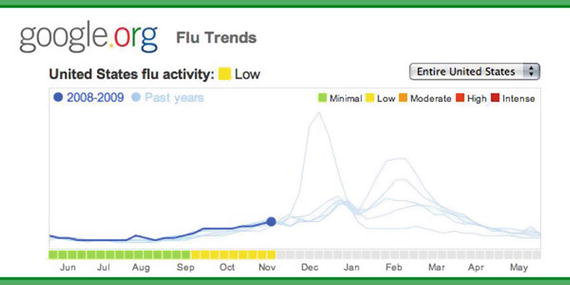
\includegraphics{google_flu}
\caption{Google Flu Trends}
\label{google_flu}
\end{figure}


Atualmente, o Google já não publica estimativas atuais de gripe e dengue com base em padrões de busca, mas continua a oferecer estimativas históricas produzidas pelo Google Flu Trends e Google Dengue Trends. Isto, principalmente devido a falta de acuracidade dos modelos de predição, evidenciados quando o algoritmo subestimou a necessidade de vacinas nos anos de 2011-2013 nos Estados Unidos  \cite{article_google_flu}.

Outras empresas também estão usando feeds de mídia social, como Facebook, Twitter e seus equivalentes, para entender as tendências em tudo, desde previsões de tendências de consumo quanto em monitoramento de tragédias. A tecnologia AI está sendo usada de muitas maneiras por essas empresas para extrair e entender os dados. Por exemplo, algumas empresas usam técnicas de processamento de linguagem natural (NLP) para interpretar o conteúdo de mídia social, enquanto outras empresas estão explorando como a análise de sentimento das mídias sociais pode ser usada para entender o que as pessoas estão postando. Os resultados atuais indicam que o uso de NLP juntamente com análise de sentimento ajuda a diferenciar entre "eu me sinto bem" e "eu me sinto mal", que se torna um grande diferencial no rastreamento de tendências de saúde \cite{book_social_machines}.
	
	\subsection*{Desafios}
Infelizmente, analisar os feeds de mídia social é muito mais difícil do que parece. Suponha que alguém escreveu um tweet "Meu médico me disse para tomar aspirina. Como eu me sinto melhor \#not ". Embora o hashtag \#not deixa claro que "me sinto melhor " é sarcástico, se removemos o hashtag, não sabemos se o escritor está sendo sério ou sarcástico.

Os sistemas atuais resolvem este problema através do acoplamento de técnicas de Machine Learning com técnicas de análise de linguagem. No entanto, a fim de serem eficientes, estas técnicas exigem um grande número de exemplos para ser "marcado" por pessoas, o que significa que as pessoas explicitamente precisam indicar recursos como sentimento e sarcasmo. Uma vez que o computador tem essas informações adicionais anotadas, resultados de pesquisas atuais indicam que o computador pode, então, mais precisamente correlacionar grandes conjuntos de dados para descobrir quais palavras prever, quais recursos e usar os resultados para analisar novos conjuntos de dados \cite{book_social_machines}.

	\section{Twitter}
	
	Twitter é uma rede social onde milhões de curtas mensagens de 140 caracteres são postadas diariamente (microblogging). Esta rede tem um crescente volume de dados graças um grande número de usuários ativos \cite{conference_twitter_alg}.

	Por ser uma ferramenta de fácil e rápida utilização, usuários utilizam a rede para comentar situações cotidianas e/ou eventos em tempo real (shows, esportes, premiações), criando o efeito de segunda tela (Tela 1: Evento ou TV, Tela 2: Smartphone conectado em redes sociais focados no assunto em si), o que tornou a rede rica em informações abrangendo diversas áreas e diversos públicos \cite{conference_twitter_sports}.

	A extração de dados dos diversos “tweets” se mostrou extremamente útil ultimamente, possibilitando saber qual é a popularidade de tópicos, e qual foi a reação dos usuários neste tópico,  ainda com a possibilidade de mapear qual é o público alvo (idade, sexo, localização, etc) pelo cadastro que é efetuado no ato de criação de um perfil na rede.

	Segundo o Twitter, em junho de 2016, ele contava com 313 Milhões de usuários \cite{twitter_company} postando em média 500 milhões de tweets por dia \cite{TwitterU87:online}.
	
	\section{ICONIX}	
	
	O ICONIX é um método de desenvolvimento de software minimalista, focado em atuar na área entre a elaboração dos casos de uso e o do código \cite{iconix}. A ênfase do método está em desenvolver uma boa análise e um bom design a partir de um processo incremental, no qual os diagramas de caso de uso são a base para cada iteração. As fases do desenvolvimento delimitadas pelo ICONIX são: Requisitos, Análise e Design Preliminares, Design Detalhado e Implementação.
	
	Na fase de Requisitos, os requisitos funcionais (que definem quais as capacidades do sistema) pré-elaborados são analisados com o intuito de realizar um modelo de domínio, um dicionário dos termos e objetos reais do seu projeto e de como eles se relacionam superficialmente. A partir do modelo de domínio, estabelecem-se os requisitos comportamentais, que detalham as ações do usuário e como o sistema deve responder a elas. \cite{iconix} Storyboads da GUI são uma ferramenta importante na idenficação destes requisitos, enquanto diagramas de caso de uso são utilizados para documentar cada cenário encontrado.
	
	Baseadas nos casos de uso encontrados, as demais fases se repetem a cada iteração, trabalhando alguns poucos casos de uso por vez. Durante a Análise e Design Preliminares, os casos de uso são refinados através de diagramas de robustez, ajudando a complementar o modelo de domínio com a identifição de classes antes ignoradas e dos atributos de cada classe. No Design Detalhado, cada caso de uso gera um diagrama de sequência de mensagens que descreve todas as chamadas de método que ocorrem entre os objetos naquele cenário. Com base nestes diagramas, o modelo de domínio é atualizado com os métodos descritos e torna-se um diagrama de classes.
	
	Quando a fase de Design Detalhado acaba, a modelagem realizada até o momento deve ser capaz de descrever com clareza o código a ser escrito. Inicia-se então a fase de Implementação. As classes descritas no diagrama de classes são geradas, seus métodos são implementados e testes unitários são escritos garantir o funcionamento do sistema. Essencialmente, você deve testar todas as funções identificadas durante a análise de robustez. \cite{iconix} Também são realizados testes de integração e aceitação. Por último, revisa-se o código e atualiza-se o modelo para se preparar para a próxima iteração.  
	
	Entre cada uma das fases, atingi-se uma milestone que consiste numa revisão crítica do que foi elaborado até o momento para assegurar que os requisitos estão sendo atendidos corretamente. A elaboração dos casos de uso, diagramas de robustez e de sequência de mensagem são a parte chamada de dinâmica no ICONIX e os diagramas de domínio e de classes são a parte estática. A figura \ref{iconix_diagram} apresenta uma visão geral do processo.
	
\begin{figure}[!htb]
\centering
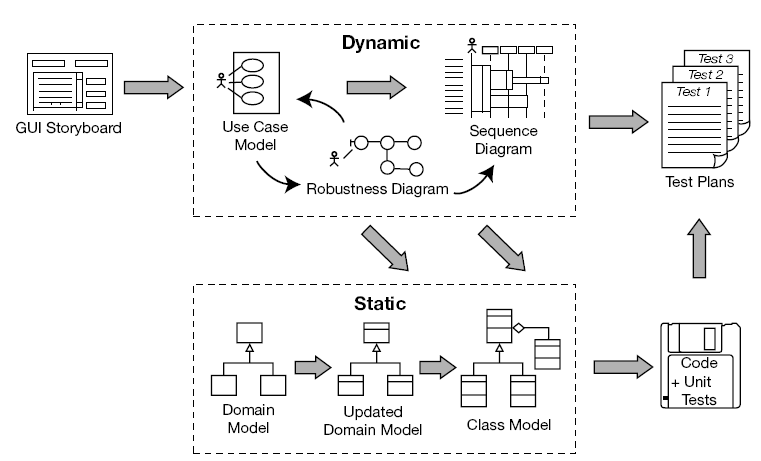
\includegraphics[scale=0.5]{iconix}
\caption{Visão Geral do Processo ICONIX \cite{iconix}}
\label{iconix_diagram}
\end{figure}

	%% Quero falar sobre TDD %%
	 
	
% ----------------------------------------------------------
% Finaliza a parte no bookmark do PDF
% para que se inicie o bookmark na raiz
% e adiciona espaço de parte no Sumário
% ----------------------------------------------------------
\phantompart

% ----------------------------------------------------------Theory and Practice
% ELEMENTOS PÓS-TEXTUAIS
% ----------------------------------------------------------
\postextual
% ----------------------------------------------------------

% ----------------------------------------------------------
% Referências bibliográficas
% ----------------------------------------------------------

\bibliography{tcc_pesquisa}
	

\end{document}
